\documentclass{article}\usepackage[]{graphicx}\usepackage[]{color}
%% maxwidth is the original width if it is less than linewidth
%% otherwise use linewidth (to make sure the graphics do not exceed the margin)
\makeatletter
\def\maxwidth{ %
  \ifdim\Gin@nat@width>\linewidth
    \linewidth
  \else
    \Gin@nat@width
  \fi
}
\makeatother

\definecolor{fgcolor}{rgb}{0.345, 0.345, 0.345}
\newcommand{\hlnum}[1]{\textcolor[rgb]{0.686,0.059,0.569}{#1}}%
\newcommand{\hlstr}[1]{\textcolor[rgb]{0.192,0.494,0.8}{#1}}%
\newcommand{\hlcom}[1]{\textcolor[rgb]{0.678,0.584,0.686}{\textit{#1}}}%
\newcommand{\hlopt}[1]{\textcolor[rgb]{0,0,0}{#1}}%
\newcommand{\hlstd}[1]{\textcolor[rgb]{0.345,0.345,0.345}{#1}}%
\newcommand{\hlkwa}[1]{\textcolor[rgb]{0.161,0.373,0.58}{\textbf{#1}}}%
\newcommand{\hlkwb}[1]{\textcolor[rgb]{0.69,0.353,0.396}{#1}}%
\newcommand{\hlkwc}[1]{\textcolor[rgb]{0.333,0.667,0.333}{#1}}%
\newcommand{\hlkwd}[1]{\textcolor[rgb]{0.737,0.353,0.396}{\textbf{#1}}}%
\let\hlipl\hlkwb

\usepackage{framed}
\makeatletter
\newenvironment{kframe}{%
 \def\at@end@of@kframe{}%
 \ifinner\ifhmode%
  \def\at@end@of@kframe{\end{minipage}}%
  \begin{minipage}{\columnwidth}%
 \fi\fi%
 \def\FrameCommand##1{\hskip\@totalleftmargin \hskip-\fboxsep
 \colorbox{shadecolor}{##1}\hskip-\fboxsep
     % There is no \\@totalrightmargin, so:
     \hskip-\linewidth \hskip-\@totalleftmargin \hskip\columnwidth}%
 \MakeFramed {\advance\hsize-\width
   \@totalleftmargin\z@ \linewidth\hsize
   \@setminipage}}%
 {\par\unskip\endMakeFramed%
 \at@end@of@kframe}
\makeatother

\definecolor{shadecolor}{rgb}{.97, .97, .97}
\definecolor{messagecolor}{rgb}{0, 0, 0}
\definecolor{warningcolor}{rgb}{1, 0, 1}
\definecolor{errorcolor}{rgb}{1, 0, 0}
\newenvironment{knitrout}{}{} % an empty environment to be redefined in TeX

\usepackage{alltt}
\usepackage{Sweave}
\usepackage{float}
\usepackage{graphicx}
\usepackage{tabularx}
\usepackage{siunitx}
\usepackage{geometry}
\usepackage{pdflscape}
\usepackage{mdframed}
\usepackage{natbib}
\bibliographystyle{..//refs/styles/besjournals.bst}
\usepackage[small]{caption}
\setlength{\captionmargin}{30pt}
\setlength{\abovecaptionskip}{0pt}
\setlength{\belowcaptionskip}{10pt}
\topmargin -1.5cm        
\oddsidemargin -0.04cm   
\evensidemargin -0.04cm
\textwidth 16.59cm
\textheight 21.94cm 
%\pagestyle{empty} %comment if want page numbers
\parskip 7.2pt
\renewcommand{\baselinestretch}{1.5}
\parindent 0pt
\usepackage{lineno}
\linenumbers

\newmdenv[
  topline=true,
  bottomline=true,
  skipabove=\topsep,
  skipbelow=\topsep
]{siderules}

%% R Script


\IfFileExists{upquote.sty}{\usepackage{upquote}}{}
\begin{document}
\noindent \textbf{\large{Rethinking False Spring Risk}}

\noindent Authors:\\
C. J. Chamberlain $^{1,2}$, B. I. Cook $^{3}$, I. Garcia de Cortazar Atauri $^{4}$ \& E. M. Wolkovich $^{1,2}$
\vspace{2ex}\\
\emph{Author affiliations:}\\
$^{1}$Arnold Arboretum of Harvard University, 1300 Centre Street, Boston, Massachusetts, USA; \\
$^{2}$Organismic \& Evolutionary Biology, Harvard University, 26 Oxford Street, Cambridge, Massachusetts, USA; \\
$^{3}$NASA Goddard Institute for Space Studies, New York, New York, USA; \\
$^{4}$French National Institute for Agricultural Research, INRA, US1116 AgroClim, F-84914 Avignon, France
\vspace{2ex}
$^*$Corresponding author: 248.953.0189; cchamberlain@g.harvard.edu\\

\renewcommand{\thetable}{\arabic{table}}
\renewcommand{\thefigure}{\arabic{figure}}
\renewcommand{\labelitemi}{$-$}
\setkeys{Gin}{width=0.8\textwidth}

%%%%%%%%%%%%%%%%%%%%%%%%%%%%%%%%%%%%%%%%%%%%%%%

\subsection*{Defining False Spring: An example in one temperate plant community - \textit{methods for calculating FSI in Harvard Forest example}}
We collected data for determining biological spring onset using three methods. The first method for was from long-term observational data recorded for 33 tree species by John O'Keefe at Harvard Forest from 1990 to 2014 \citep{OKeefe2014}. Budburst was definied as 50\% green tip emergence. We subsetted this dataset to include only the tree species that were most consistently observed, which ended up being eight species. The second dataset was from PhenoCam data, which are field cameras placed in the Harvard Forest canopy that take real-time images of plant growth and are programmed to record initial green up. The final set was collected through the USA National Phenology Network (USA-NPN), using their Data Visualization tool to gather Extended Spring Index values (SI-x) by accessing the "Spring Indices, Historic Annual" gridded layer and looking specifically at "First Leaf - Spring Onset" \citep{SI-x2016}. The SI-x value uses the time of leaf out using historical dates of budburst from honeysuckle and lilac clones around the U.S. and combines that information with daily recordings from local weather stations \citep{USA-NPN2016, Ault2015, Ault2015a, Schwartz2013, Schwartz1997}. Through assessing past years' weather and budburst, scientists are able to determine general weather trends that subsequently lead to leaf out. Based on these trends, SI-x values can be calculated from daily weather data \citep{USA-NPN2016}.
\par
The date of last spring freeze was gathered from the Fisher Meteorological Station which was downloaded from the Harvard Forest web page (data available online\footnote{http://harvardforest.fas.harvard.edu/meteorological-hydrological-stations}). The $T_{min}$ values were used and the last spring freeze was determined from the latest spring date that the temperature reached -2$^{\circ}$C or below. 
\par
PhenoCam data is not available for Harvard Forest until 2008 and observation data is only recorded through 2014, so this evaluation assesses FSI values from 2008 through 2014.
The FSI values were calculated for each methodology using the formula based on the study performed by Marino et al. (2011).  

\subsection*{How Species' Phenological Cues Shape Vegetative Risk - \textit{methods for experiment}}
Data from a growth chamber experiment was used (Flynn \& Wolkovich, 2018) to assess the phenological cue interaction with the duration of vegetative risk. Cuttings for the experiment were made in January 2015 for 9 species at Harvard Forest (HF, 42.5$^{\circ}$N, 72.2$^{\circ}$W) and the Station de Biologie des Laurentides in St-Hippolyte, Qu\'ebec (SH, 45.9$^{\circ}$N, 74.0$^{\circ}$W). The experiment examined the 9 temperate trees and shrubs using a fully crossed design of three levels of chilling (field chilling, field chilling plus 30 days at either 1 or 4 $^{\circ}$C), two levels of forcing (20$^{\circ}$C/10$^{\circ}$C or 15$^{\circ}$C/5$^{\circ}$C day/night temperatures) and two levels of photoperiod (8 versus 12 hour days) resulting in 12 treatment combinations. Observations on the phenological stage of each cutting was made every 2-3 days over 82 days. Phenology was assesed using a BBCH scale that was modified for trees \citep{Finn2007}. We used the same statistical analyses as the original study: mixed-effects hierarchical models warming, photoperiod, and chilling treatments, and all two-way interactions as predictors and species as modeled groups.


\subsection*{Predictable Regional Differences in Climate, Species Responses and False Spring Risk - \textit{climate data and phenology data}}
We analyzed five archetypal regions across North America and Europe. We collected phenology data through the USA National Phenology Network (USA-NPN), using their Data Visualization tool to gather Extended Spring Index values (SI-x) by accessing the "Spring Indices, Historic Annual" gridded layer and looking specifically at "First Leaf - Spring Onset" \citep{SI-x2016}. We looked at each SI-x value for each North American site (i.e. Waterville, ME, Yakima, WA, and Reidsville, NC) from 1981-2016 to evaluate the spread of spring onset dates for those regions. For the European sites (i.e. Bamberg, Germany and Lyon, France) we used phenology observation studies that assessed multiple years of \textit{in situ} budburst dates for the dominant species in those regions \citep{Soudani2012, White2009,Schaber2005}. We then collected climate data by downloading Daily Summary climate datasets from the NOAA Climate Data Online tool (data available online\footnote{https://www.ncdc.noaa.gov/cdo-web/search?datasetid=GHCND}). Each location assesses 50 years of climate data. We then calculated the number of years that fell below -2.2$^{\circ}$C within the budburst date range for each region. 

\newpage
\subsection*{Supplemental Figures}

\begin{figure}[H]

{\centering 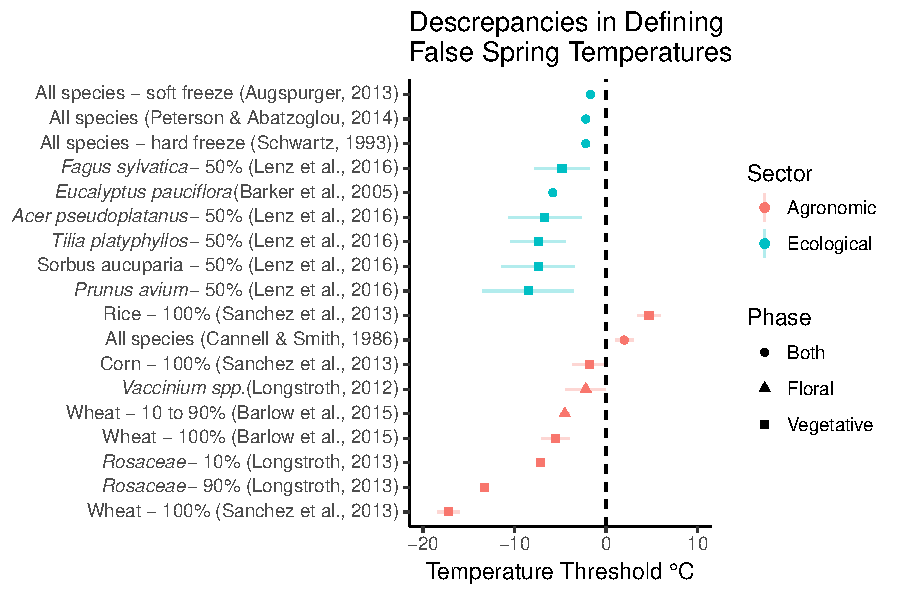
\includegraphics[width=\maxwidth]{figure/temp-1} 

}

\caption[A comparison of damaging spring freezing temperature thresholds across ecological and agronomic studies]{A comparison of damaging spring freezing temperature thresholds across ecological and agronomic studies. Each study is listed on the y axis along with the taxonimic group of focus. Next to the species name is the freezing definition used within that study (e.g. 100\% is 100\% lethality). Each point is the best estimate recorded for the temperature threshold with standard deviation if indicated in the study. The shape of the point represents the phenophases of interest and the colors indicate the type of study (i.e. agronomic or ecological).}\label{fig:temp}
\end{figure}



\newpage
\nocite{Schwartz1993}
\nocite{Barker2005}
\nocite{Sanchez2013}
\nocite{Longstroth2012}
\nocite{Barlow2015}
\nocite{Longstroth2013}
\bibliography{..//refs/SpringFreeze.bib}

\end{document}
